
\section{Higher-Order Test Cases}
\label{sc:ho-tests}

The higher-order test cases are designed to test various aspects of higher-order dycores.
By default they use the Glissade dycore with the Blatter-Pattyn approximation 
(see Section~\ref{sc:glissade-blatter-pattyn}).
As other higher-order dycores become available, they can be applied
to these same tests. Additional test cases will be added as needed.

% =====================================
\subsection{Dome}
% =====================================
The dome test case is based on a parabolic dome of ice, similar to the Halfar test case.
By default the dome has the same radius and center thickness as the Halfar case.
However, it uses a simple square root function to define thickness as a function 
of distance from the dome center, resulting in a somewhat steeper profile.  
The dome test has been widely used for day-to-day testing
because it is simple and relatively fast to run.  It is a good test
to confirm that basic higher-order model physics is working correctly, but does
not strenuously test the physics and boundary conditions, or analytically verify the model.

\subsubsection{Provided files}

\begin{itemize}
	\item README.md \\
		Information about the test case, including technical details about running it.
	\item runDome.py \\
		The script to set up and run the test.
 	 \item dome.config \\
  		The default configuration settings for running CISM with the test case.
  	\item dome-forcing.config \\
  		An example configuration script that can be used to generate a forcing file and run CISM with it.
\end{itemize}

\subsubsection{Running the test}
One script sets up the initial condition and runs the model:

\texttt{./runDome.py}\\

\noindent
There is no script for analyzing the results.
%\textit{Optional: Time-dependent forcing example} \\

\par
The dome test case can also be used to set up an example of CISM's time-dependent
forcing capability.  (See Section \ref{io-config} for details.) By passing the runDome.py script a config file which has [CF Forcing] section, as found in dome-forcing.config,
it will generate a dome.forcing.nc file that contains time-varying fields and then run CISM using this generated netCDF file. Run:


\texttt{./runDome.py -c dome-forcing.config}\\


\subsubsection{Results}
There is not an analytic solution for this test, nor is there a script to analyze
the results.  You can manually inspect the results using a tool such as \texttt{ncview}.\footnote{See section \ref{sec:install-netcdf}}
Sample output is shown in Figure \ref{fig:domeresults}.
\begin{figure}[H]
	\centering
	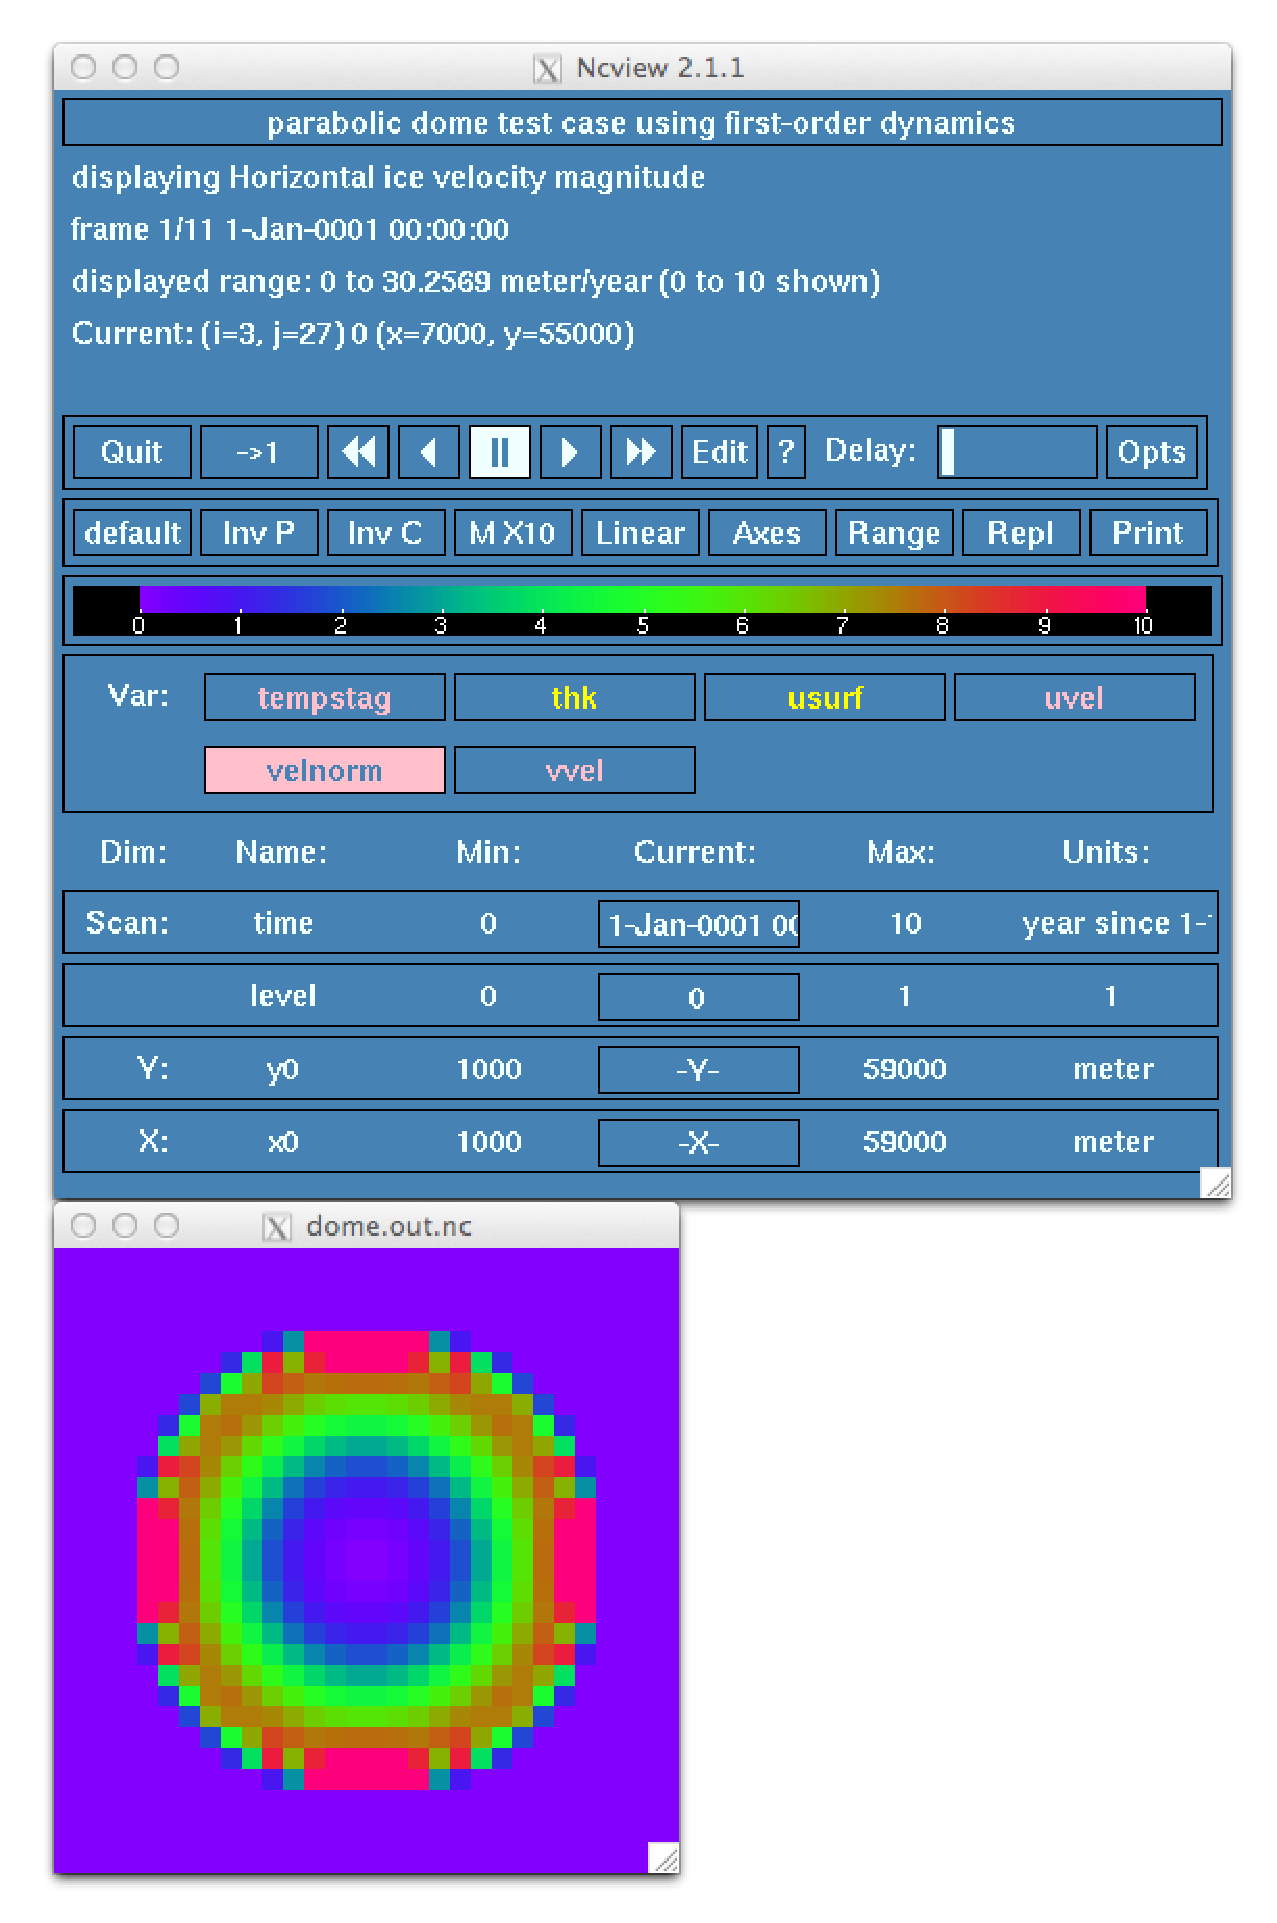
\includegraphics[width=7.0cm]{\dir/dome-output.eps}
	\caption{Dome \texttt{velnorm} (i.e., the ice speed in m/yr) field at time 0 using default \texttt{dome.config} settings. This figure is a screenshot of ncview.}
	\label{fig:domeresults}
\end{figure}
\FloatBarrier

% =====================================
\subsection{ISMIP-HOM}
% =====================================
The Ice Sheet Model Intercomparison Project for Higher-Order Models (ISMIP-HOM)
prescribes a set of experiments for testing the implementation of higher-order physics.  
For more information, see 
\href{http://homepages.ulb.ac.be/~fpattyn/ismip/}{here}\footnote{http://homepages.ulb.ac.be/\textasciitilde{}fpattyn/ismip/} 
and the ISMIP-HOM description paper by \citet{Pattyn2008}.

The python scripts provided (runISMIP\_HOM.py and plotISMIP\_HOM.py, referred to here as the ISMIP-HOM 
scripts) were created to run experiments A through F using CISM and compare the results with results from other models. 

Note: The \texttt{README.md} file gives many additional details about running and analyzing the
test case that are not described here.

\subsubsection{Provided files}

\begin{itemize}
	\item README.md \\
		Information about the test case, including technical details about running it.
	\item ismip-hom.config \\
		A default configuration file used as a template for generating the .config file for each test.
    		If you wish to run the tests with different solver settings, for example, you should edit this file.
	\item runISMIP\_HOM.py \\
		The script used for running any/all of the ISMIP-HOM experiments.  
    		Invoke with `-{}-help' to see the many command line options for controlling execution.
  \item plotISMIP\_HOM.py \\
		The script used for analyzing/plotting any/all of the ISMIP-HOM experiments.  
    		Invoke with `-{}-help' to see the many command line options for controlling execution.
\end{itemize}

\subsubsection{Running the test}
One script sets up the initial condition and runs the model:

\texttt{./runISMIP\_HOM.py}

\noindent
and another is used to analyze the results:

\texttt{./plotISMIP\_HOM.py}

\subsubsection{Results}
The \texttt{plotISMIP\_HOM.py} script will plot results relative to other models.
None of the ISMIP-HOM tests have a useful analytic solution, so these tests are
used as community benchmarks rather than actual model verification tests.
The \citet{Pattyn2008} paper is useful for intepreting model results.
An example output plot is shown in Figure \ref{fig:ismiphom-results}.

\begin{figure}[H]
	\centering
	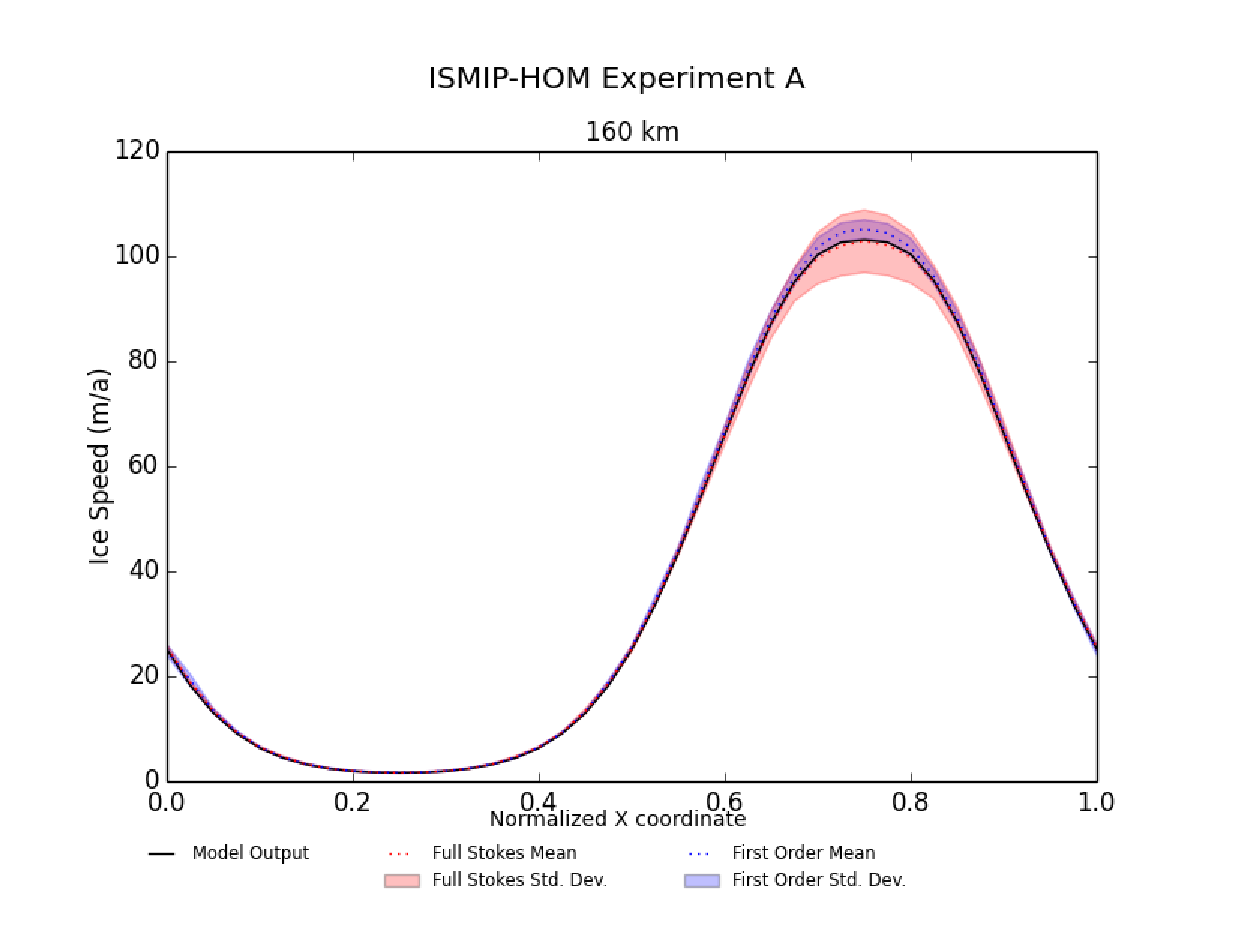
\includegraphics[width=10.0cm]{\dir/ISMIP-HOM-A-cis1.eps}
	\caption{An example of the ISMIP-HOM test case output for test A at size L=160 km. 
CISM output is shown with a black line, and the range of output from other models is shown by colored bars. 
This figure was generated with \texttt{./plotISMIP\_HOM.py -e a -s 160} after running the test with \texttt{./runISMIP\_HOM.py -e a -s 160}.
Additional options (e.g., running and plotting for multiple tests simultaneously) are described in the \texttt{README.md} and by invoking the
`-{}-help' option at the command line.}
	\label{fig:ismiphom-results}
\end{figure}
\FloatBarrier

% =====================================
\subsection{Stream}
% =====================================
\label{sc:stream_test}
The stream test case simulates flow over an idealized ice stream underlain by a subglacial till with a known and specified
yield stress distribution (see discussion in Section \ref{sc:higher-order-bcs}). For the two yield stress distributions specified in this test case, 
analytical solutions are available from \citet{Raymond2000} and \citet{Schoof2006}. 

For the Raymond test case, the yield stress within the ice stream is given a uniform value below the driving stress, and outside the
ice stream it is given a uniform value much higher than the driving stress (i.e., the yield stress distribution is approximated by a
step function). For the Schoof test case, the till yield stress across the ice stream is given by a continuously varying function.

In both cases, the basal properties vary in the across-flow direction only and are symmetric about the ice stream centerline.
As a result, the velocity solutions are also uniform along flow and symmetric about the centerline.

\subsubsection{Provided files}

\begin{itemize}
	\item README.md \\
		Information about the test case, including technical details about running it.
	\item runStream.py \\
		The script to set up and run the test.
	\item stream.config \\
  The default configuration settings for running CISM with the test case. Note that this
  file is parsed by the runStream.py script. Most of the relevant options that might be changed
  for this test case (e.g., grid spacing) can be done so from the command line, without having to
  edit the .config files (use \texttt{./runStream.py --help} for a description of available options).
  The choice of yield stress distribution (Raymond or Schoof) can be toggled
  by editing line 122 of \texttt{runStream.py}.
\end{itemize}

\subsubsection{Running the test}
One script sets up the initial condition and runs the model:

\texttt{./runStream.py}

\noindent
and another is used to analyze the results:

\texttt{./plotStream.py}

\subsubsection{Results}
The \texttt{plotStream.py} script will plot model output relative to the analytical solutions
in \citet{Raymond2000} and \citet{Schoof2006}. The choice of analytical solution for comparison
is automatic, based on the yield stress chosen in the runStream.py script. 
Figure \ref{fig:stream-results} shows example output for both test cases.

Note: The excellent agreement between the CISM results and the Raymond analytical solution
requires setting \texttt{which\_ho\_assemble\_beta = 1} in the config file
(see Section~\ref{ug.sec.config}). With this setting, the step change in yield
stress is well resolved. Otherwise there is some smoothing of the traction 
parameter $\beta$ over neighboring nodes during finite-element assembly
(Section~\ref{sec:glissade-assembly}), and the results are less accurate.
 
	
\begin{figure}[H]
  \begin{center}
	\includegraphics[width=10.0cm]{\dir/stream_raymond.eps}
	\includegraphics[width=10.0cm]{\dir/stream_schoof.eps}
  \end{center}
  \caption{Comparison between CISM model output (black) and analytic solution (red) for the Raymond (top) and Schoof (bottom) stream test cases. This figure was generated with \texttt{./plotStream.py} after running the test with \texttt{./runStream.py}.
Additional runtime options are described in the \texttt{README.md} and by invoking the `-{}-help' option at the command line.}
  \label{fig:stream-results}
\end{figure} 

% =====================================
\subsection{Confined shelf}
% =====================================
The confined shelf test is based on tests 3 and 4 of the idealized (i.e., not Ross) EISMINT shelf test 
cases.  It simulates the flow within an idealized, 500 m thick ice shelf in a 
confined, rectangular embayment.  Grounded ice is not explicitly modeled but included in the 
model setup as Dirichlet boundary conditions for velocity along the ice shelf edges.
More detailed information on this test case can be found 
\href{http://homepages.vub.ac.be/~phuybrec/eismint/iceshelf.html}{here}
\footnote{http://homepages.vub.ac.be/\textasciitilde{}phuybrec/eismint/iceshelf.html} in the 
``shelf-descr.pdf" document.

Note that the confined shelf and circular shelf experiments are both in the 
\texttt{tests/higher-order/shelf} directory and share some files.

\subsubsection{Provided files}

\begin{itemize}
	\item README.md \\
		Information about the test case, including technical details about running it.
	\item runShelfConfined.py \\
		The script to set up and run the test.
	\item shelf-confined.config \\
  The default configuration settings for running CISM with the test case.
\end{itemize}

\subsubsection{Running the test}
One script sets up the initial condition and runs the model:

\texttt{./runShelfConfined.py}

\subsubsection{Results}
There is no script for analyzing the results.  See the URL above for information 
about assessing the model output.
You can manually inspect the results using a tool such as \texttt{ncview}.
Figure \ref{fig:confinedshelf-results} shows an example.

\begin{figure}[H]
	\centering
	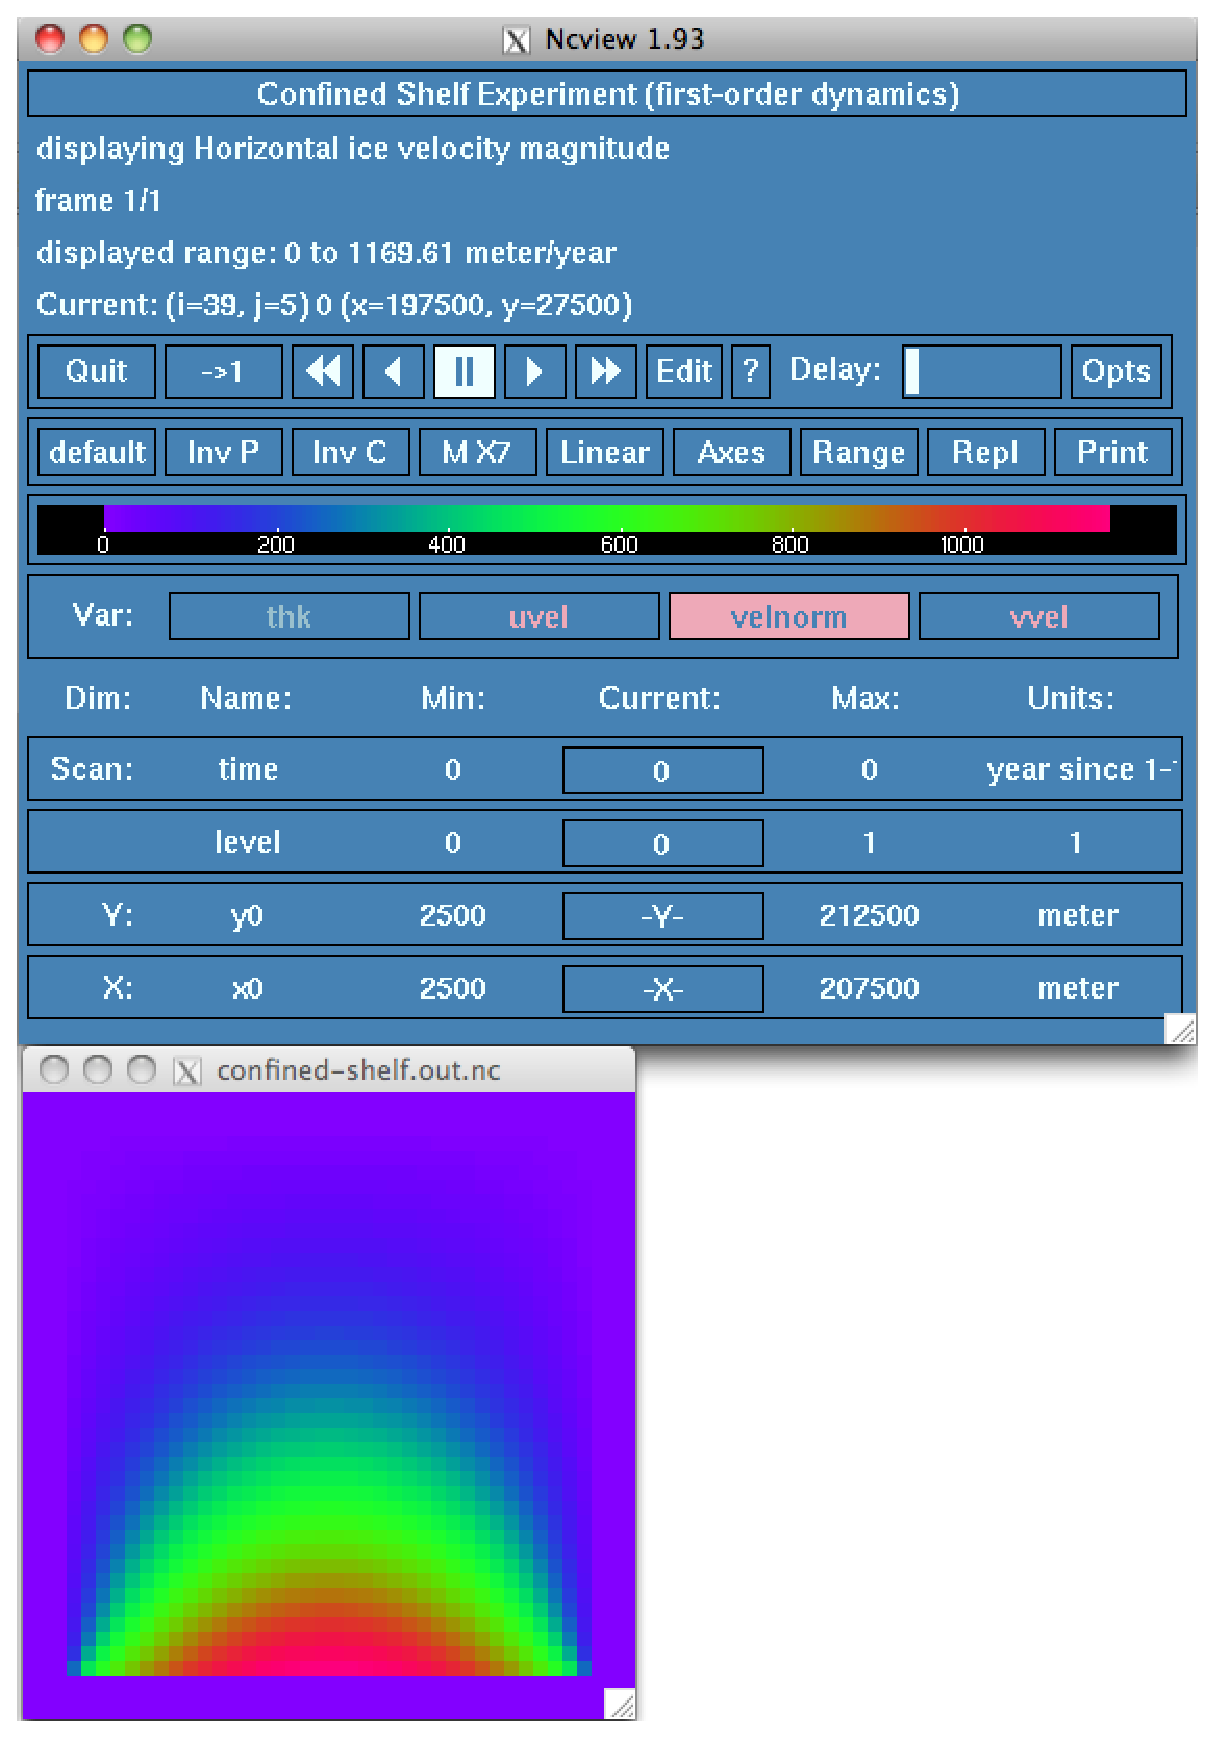
\includegraphics[width=8.0cm]{\dir/confinedshelf-output.eps}
	\caption{Confined shelf \texttt{velnorm} field using default \texttt{shelf-confined.config} settings. This figure is a screenshot of ncview.}
	\label{fig:confinedshelf-results}
\end{figure}
\FloatBarrier

% =====================================
\subsection{Circular shelf}
% =====================================
The circular shelf test case is a variant on the confined shelf discussed above. It simulates the flow within a circular ice shelf with a uniform thickness
of 1000 m, which is grounded at a single grid point at its center. This test case confirms a working ``floating ice" boundary condition
in 2D (i.e., in map plane view) and also confirms radial symmetry. 

Note that the confined shelf and circular shelf experiments are both in the 
\texttt{tests/higher-order/shelf} directory and share some files.

\subsubsection{Provided files}

\begin{itemize}
	\item README.md \\
		Information about the test case, including technical details about running it.
	\item runShelfCircular.py \\
		The script to set up and run the test.
	\item shelf-circular.config \\
          The default configuration settings for running CISM with the test case.
\end{itemize}

\subsubsection{Running the test}
One script sets up the initial condition and runs the model:

\texttt{./runShelfCircular.py}

\subsubsection{Results}
There is no  script for analyzing the results.
You can manually inspect the results using a tool such as \texttt{ncview}.
Figure \ref{fig:circularshelf-results} shows an example.

\begin{figure}[H]
	\centering
	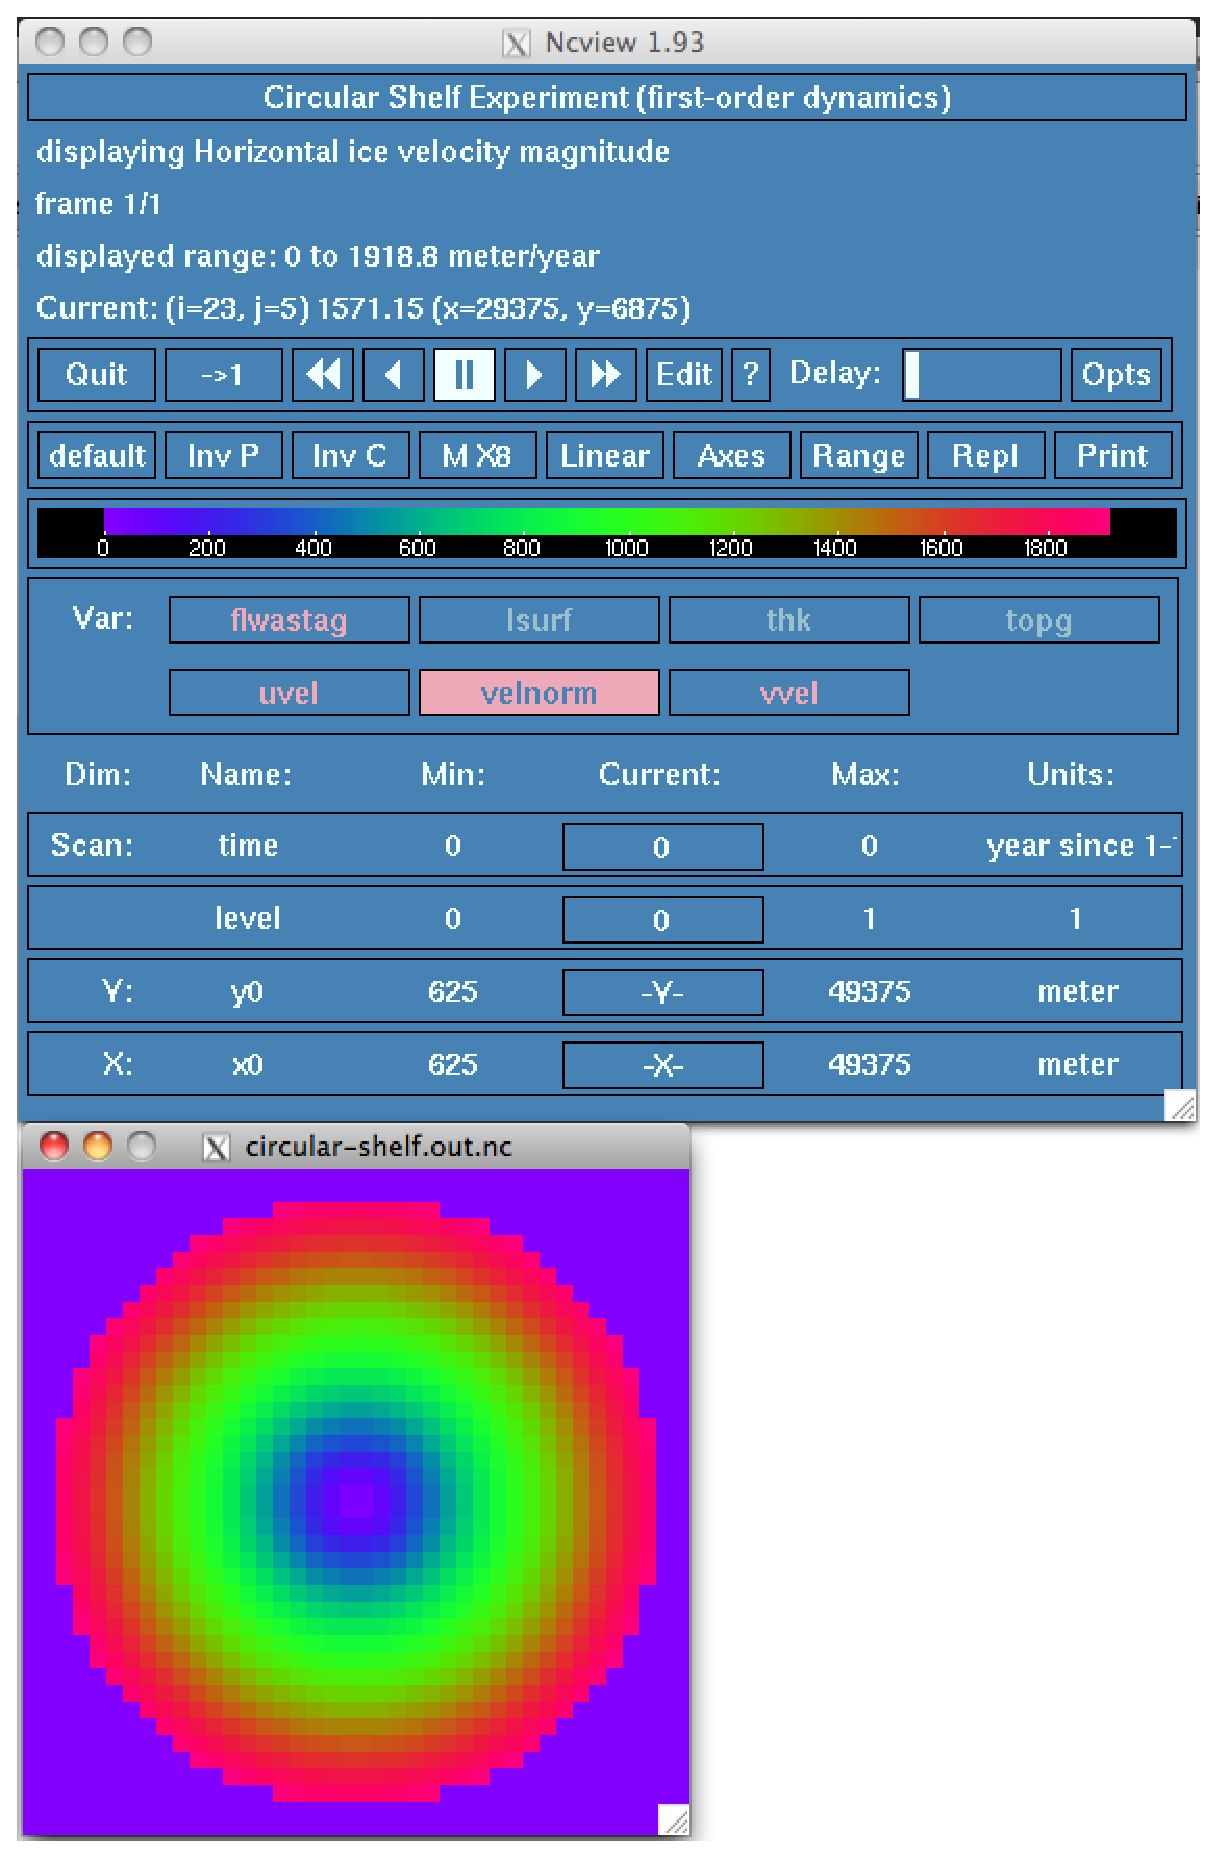
\includegraphics[width=8.0cm]{\dir/circularshelf-output.eps}
	\caption{Circular shelf velnorm field using default \texttt{shelf-circular.config} settings. This figure is a screenshot of ncview.}
	\label{fig:circularshelf-results}
\end{figure}
\FloatBarrier

% =====================================
\subsection{Ross Ice Shelf}
\label{sc:ross_test}
% =====================================
The Ross experiment is designed to simulate the flow of the Ross Ice Shelf of Antarctica under idealized conditions (e.g., constant and uniform
flow-law rate factor). For more information about the experiment and its results, see 
\href{http://homepages.vub.ac.be/~phuybrec/eismint/iceshelf.html}{here}\footnote{http://homepages.vub.ac.be/\textasciitilde{}phuybrec/eismint/iceshelf.html}. 
Also, see \citet{MacAyeal:1996vn} for a discussion of the official model intercomparison results.

Using the Glissade solver with the Blatter-Pattyn approximation, this experiment typically 
takes about 10 minutes to run on a single processor.  Using the shallow-shelf approximation instead,
the results are very similar and are found more quickly (in less than a minute).
For this reason, the SSA (\texttt{which\_ho\_approx = 1}) is the default.

\subsubsection{Provided files}

\begin{itemize}
	\item README.md \\
		Information about the test case, including technical details about running it.
	\item runRoss.py \\
		The script to set up and run the test.
	\item ross.config \\
  The default configuration settings for running CISM with the test case.
	\item plotRoss.py \\
		The script to plot the test results.
\end{itemize}

\subsubsection{Running the test}
One script sets up the initial condition and runs the model:

\texttt{./runRoss.py -r}

\noindent
(Without the ``-r'' flag, the script will set up the initial condition but not run CISM.)
Another script can be used to visualize the results:

\texttt{./plotRoss.py}

\subsubsection{Results}
The \texttt{plotRoss.py} script will generate a figure of the velocity field
calculated for the Ross Ice Shelf.  The results should look very similar to Figures \ref{fig:rossresults1} and \ref{fig:rossresults2}. You can
compare these with similar figures in the paper by \citet{MacAyeal:1996vn}.

\begin{figure}[H]
	\centering
	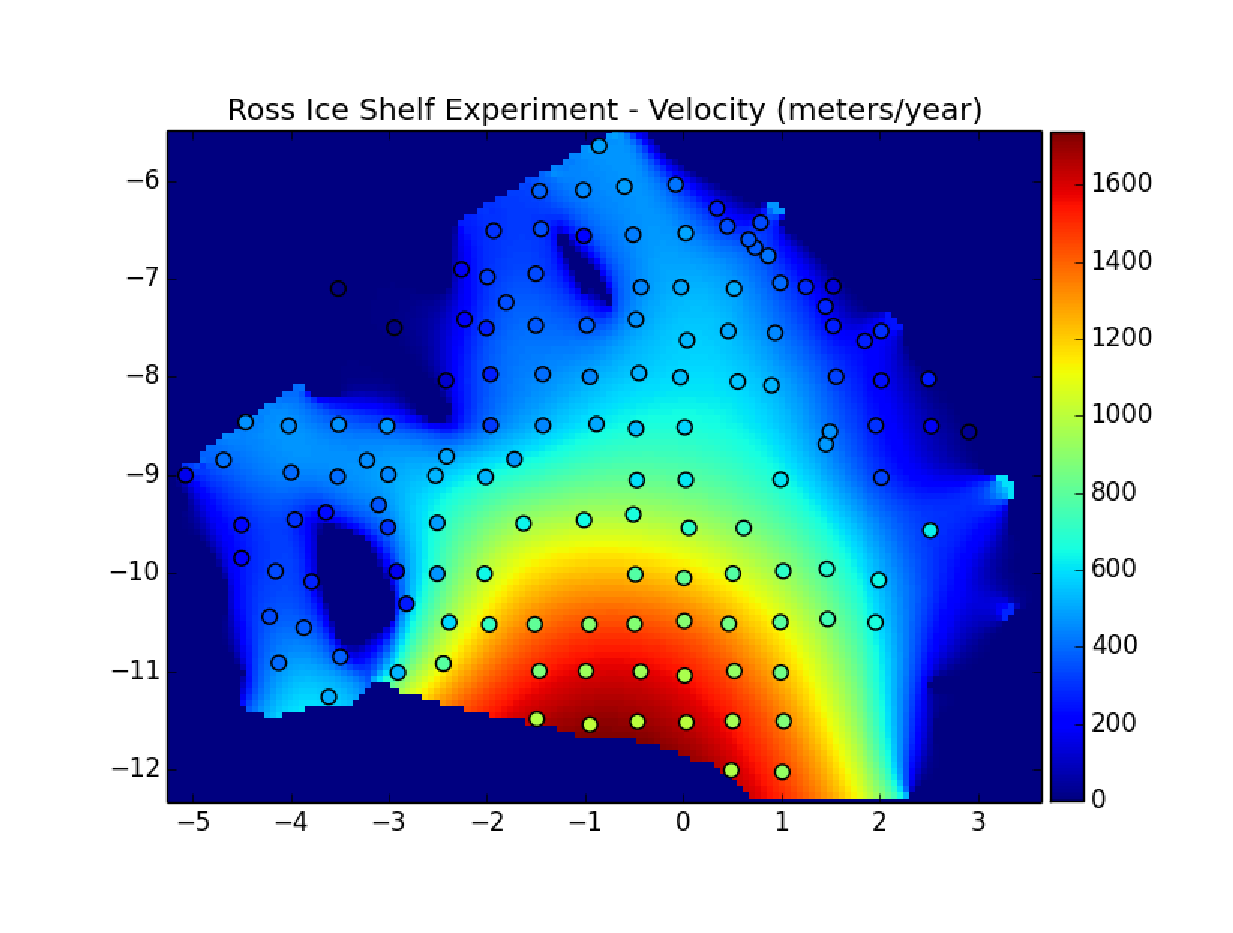
\includegraphics[width=10.0cm]{\dir/RossModelVelField.eps}
	\caption{Ross Ice Shelf velocity field calculated by CISM. This figure is generated by \texttt{plotRoss.py}.}
	\label{fig:rossresults1}
\end{figure}
%\FloatBarrier

\begin{figure}[H]
	\centering
	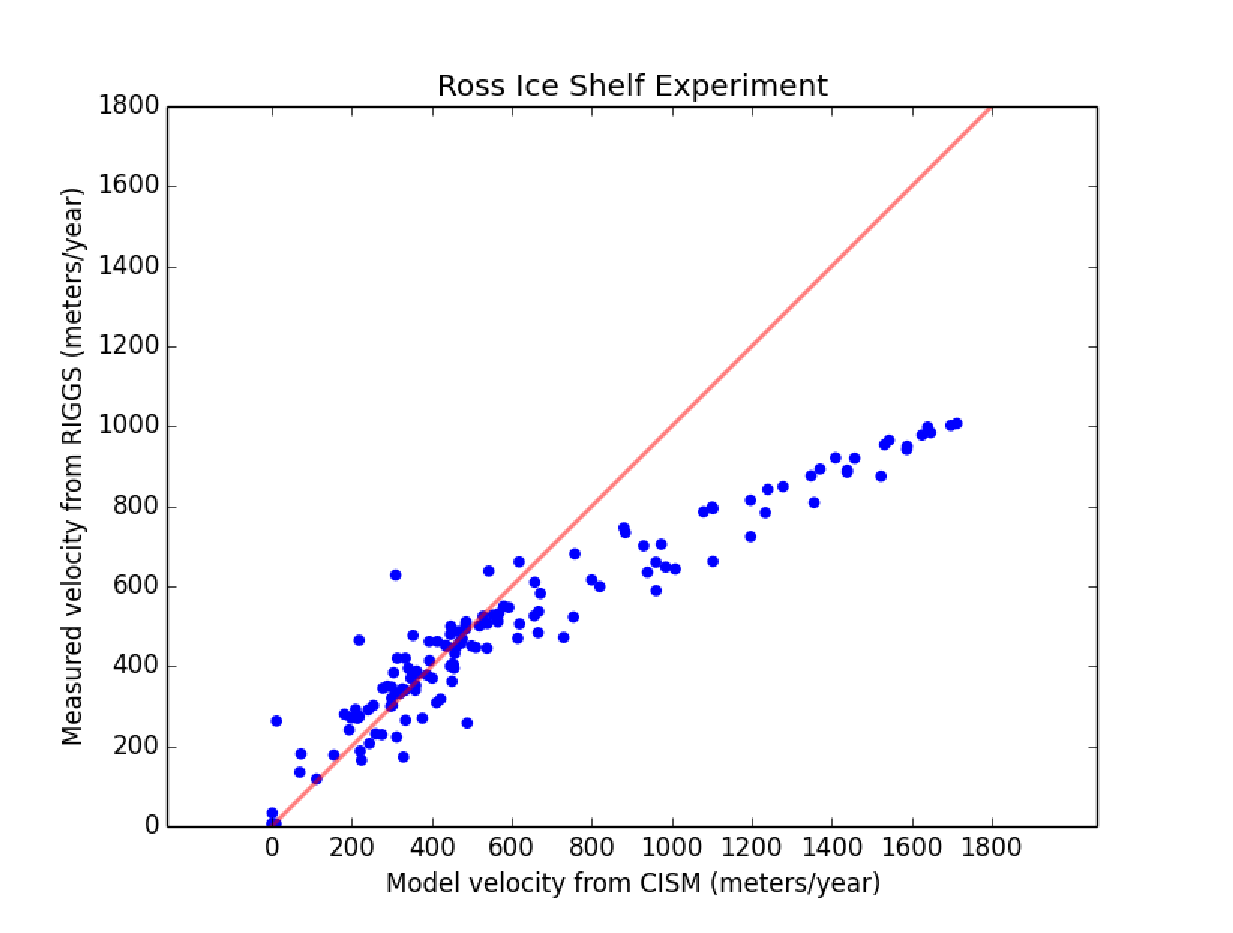
\includegraphics[width=10.0cm]{\dir/RossModelvsObs.eps}
	\caption{CISM-modeled Ross Ice Shelf speeds vs. those from observations. This figure is generated by \texttt{plotRoss.py}.}
	\label{fig:rossresults2}
\end{figure}
\FloatBarrier


% =====================================
\subsection{MISMIP}
\label{sc:mismip}
% =====================================
The MISMIP (Marine Ice Sheet Model Intercomparison Project) experiments \citep{Pattyn2012} are designed to study the behavior of marine ice-sheet models under idealized conditions while modifying the flow-rate factor. The goal is to study the advance and retreat of the ice sheet and ideally, for a set flow-rate factor, the grounding line position should be the same in the advance state as in the retreat state. \citet{Pattyn2012} and \citet{Leguy2014} showed the conditions under which the hysteresis is minimal while using different resolution, Stokes approximations and basal water pressure at the grounding line. 
Using the Glissade solver with the SSA approximation, this experiment typically takes about a couple of hours to run on 36 processors and at a resolution of 8~km. While running with a linear bed, the initial time step should be chosen as 1~y for the first 3 flow rate values and can then be relaxed to 2~ and 4~yr later on. Of course this will vary based on the chosen resolution.

\subsubsection{Provided files}

\begin{itemize}
	\item README.mismip \\
		Information about the test case, including technical details about running it.
	\item mismipSetup.py \\
		The script to set up the test.
	\item mismipRun.py \\
		The script to run the test.
	\item mismipWriteGL.py \\
		The script to write the file containing the grounding line location.
	\item mismipPlotGL.py \\
		The script to plot the test results.		
	\item mismip.config.template \\
		The default configuration template settings for running CISM with the test case. Inputs will vary based on the options used with the setup file. 
	\item runCISM.cheyenne.template \\
		The template script to submit a job on Cheyenne HPC system. The wall time, number of nodes and processors will need to be adjusted depending on the need of the simulation. 
\end{itemize}

\subsubsection{Running the test}
For detailed instruction, follow the instruction from the \texttt{README.mismip} file. In short the order of operations are:
Set up the experiment (add options if need be):

\texttt{> python mismipSetup.py}

\noindent
Run the experiment (add options if need be):

\texttt{> python mismipRun.py}

\noindent
Write the grounding line position to a file (add options if need be):

\texttt{> python mismipWriteGL.py}

\noindent
Plot the results (add options if need be):

\texttt{> python mismipPlotGL.py}


\subsubsection{Results}
The \texttt{mismipPlotGL.py} script will generate a figure of the grounding line position as a function of the flow-rate factor at the end of each experiment and the semi-analytic solution from \citet{Schoof2007}.
The results should look very similar to Figures \ref{fig:mismiplinear} (for the linear bed) and \ref{fig:mismippoly} (for the polynomial bed) when using the a powerlaw basal friction. You can compare these with similar figures in the papers by  \citet{Pattyn2012} and \citet{Leguy2014}.

\begin{figure}[H]
	\centering
	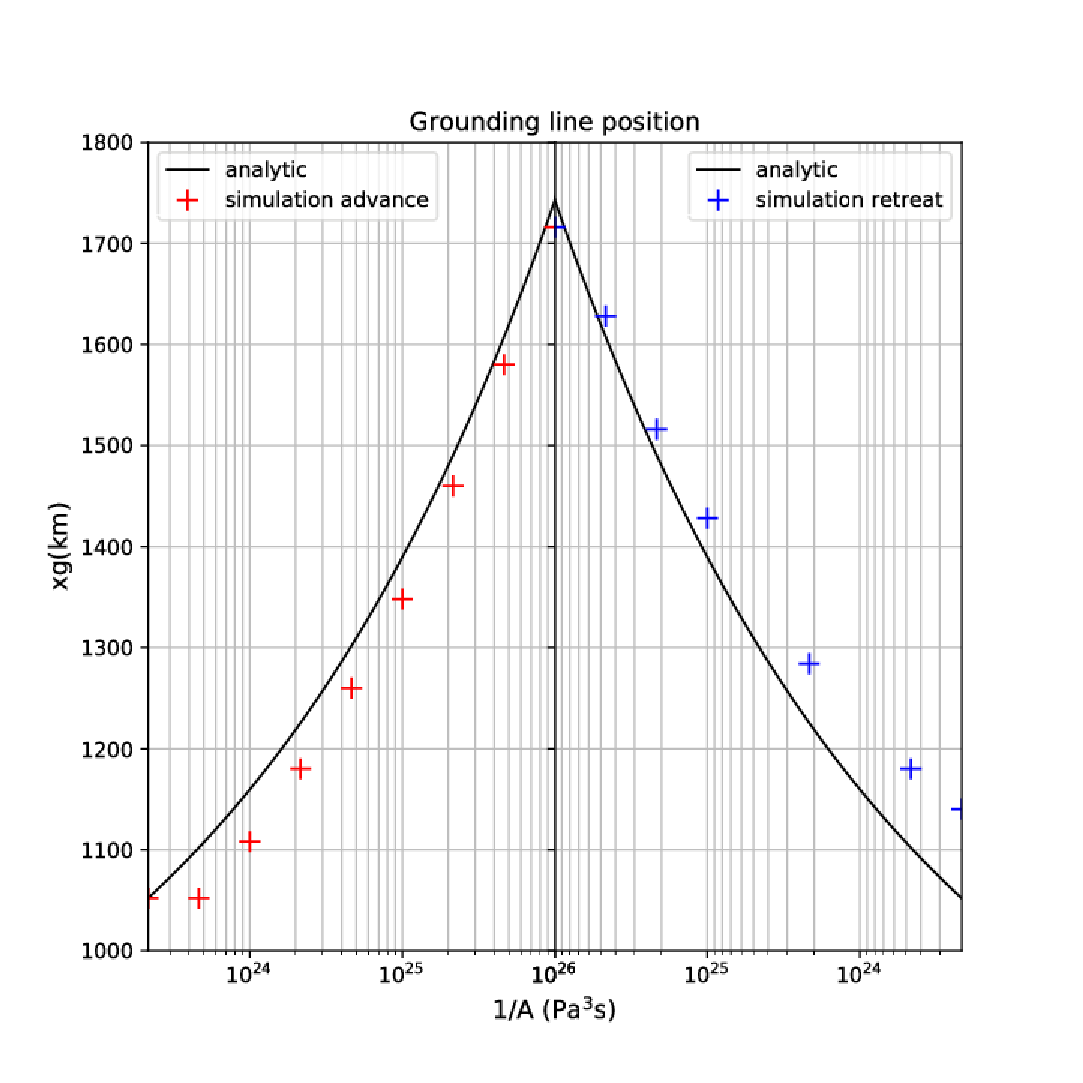
\includegraphics[width=10.0cm]{\dir/mismiplinear.eps}
	\caption{Steady state grounding line position calculated by CISM for the MISMIP experiment over a linear bed topography. This figure is generated by \texttt{mismipPlotGL.py}.}
	\label{fig:mismiplinear}
\end{figure}

\begin{figure}[H]
	\centering
	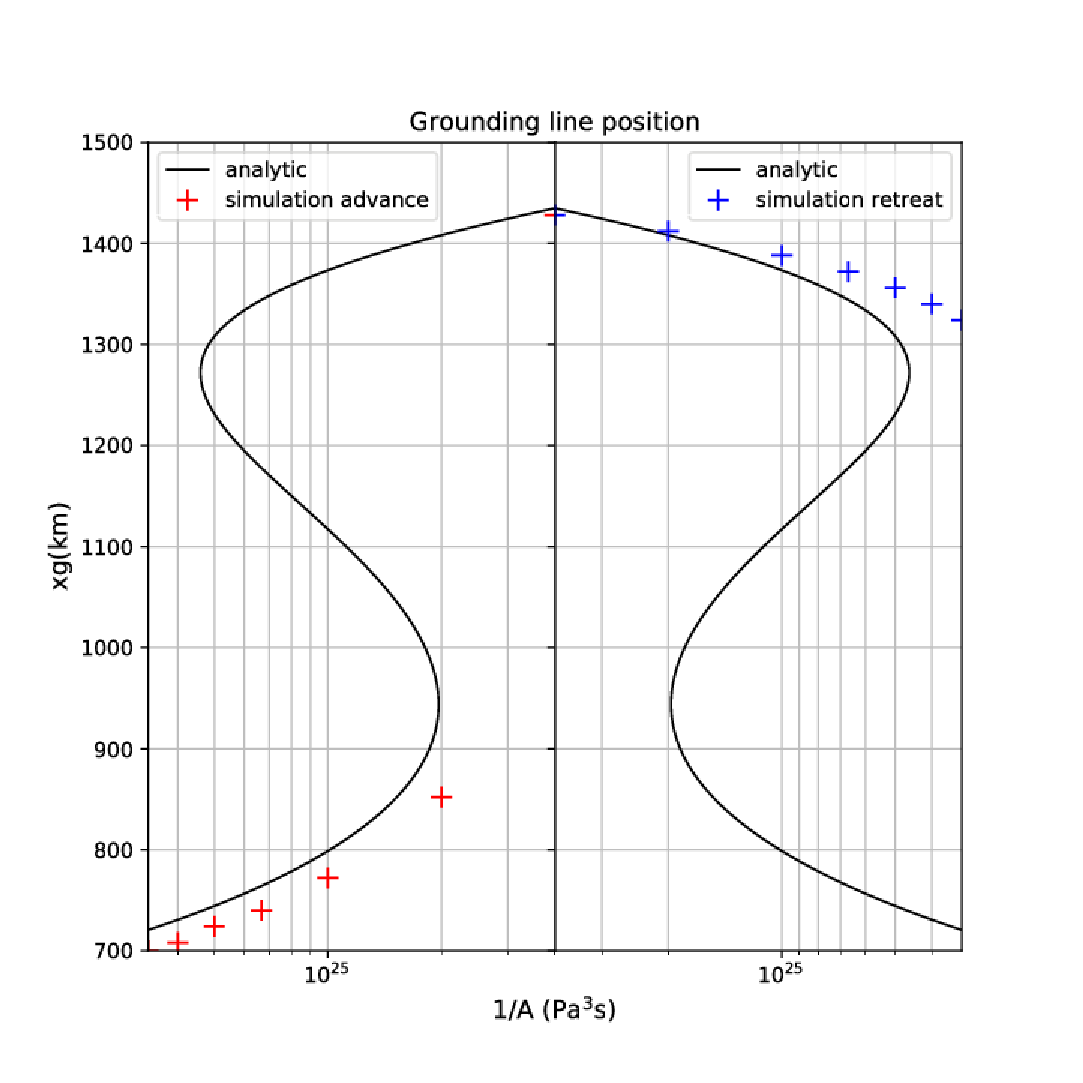
\includegraphics[width=10.0cm]{\dir/mismippoly.eps}
	\caption{Steady state grounding line position calculated by CISM for the MISMIP experiment over a polynomial bed topography. This figure is generated by \texttt{mismipPlotGL.py} using the option \texttt{--bed poly}.}
	\label{fig:mismippoly}
\end{figure}


% =====================================
\subsection{MISMIP3d}
\label{sc:mismip3d}
% =====================================
The MISMIP3d (Marine Ice Sheet Model Intercomparison Project) experiments \citep{Pattyn2013} are designed to study the transient behavior of marine ice sheet model 


% =====================================
\subsection{MISOMIP}
\label{sc:misomip}
% =====================================
The MISOMIP (Marine Ice Sheet Model Intercomparison Project) experiments \citep{AsayDavis2016} are designed to study the transient behavior of marine ice sheet model 


% =====================================
\subsection{Other tests}
% =====================================
Other higher-order tests that are still in development (e.g., ``slab") are also included in the \texttt{./tests/}
directory. Instructions for running these tests are included in each directory. Since these tests have not yet been validated, 
they are for use at your own risk.

% ==============================================
\section{The build and test structure (BATS)}
\label{sc:bats}
% ==============================================
A build and test structure (BATS) has been included in the \texttt{./tests/regression/} directory. BATS is capable of
automatically building CISM and then running a set of regression tests on a number of platforms. BATS is primarily
intended to allow users and developers of CISM to quickly generate a set of regression tests for use with the
\href{https://github.com/LIVVkit/LIVVkit}{Land Ice Verification and validation toolkit(LIVVkit)}
\footnote{https://github.com/LIVVkit/LIVVkit}. This allows users to quickly and easily build
confidence in their installation of CISM and, by extension, their scientific results. 

\subsubsection{Provided files}

\begin{itemize}
	\item README.md \\
		Information about the build and test structure, including technical details about using it.
    \item \texttt{build\_and\_test.py} \\
		The main script to build CISM, and run a set of regression tests.
    \item \texttt{setup\_hopper.bash} and \texttt{setup\_titan.bash} \\
        Scripts to load the needed modules on the higher-performance-computing architectures Hopper (NERSC) and Titan
        (OLCF).
    \item \texttt{util/} \\
        A directory containing a set of helper python modules and files for \texttt{build\_and\_test.py}.
\end{itemize}

\subsubsection{Using BATS} 

BATS works very similar to how you would build CISM and run one or more CISM tests. BATS will
build a version of CISM, and then either run a set of regression tests if you are using a personal computer (PC), or
setup a series of regression tests and generate a job submission script if you are using a high-performance-computing
architecture (HPC). 

\par
For example, on the HPC Titan, if you wanted to build CISM using the gnu compiler, and run a set of regression tests,
you would run these commands: 

\begin{verbatim}
cd tests/regression/
source setup_titan.bash
./build_and_test.py -p titan -c gnu -b ./build
\end{verbatim}

\noindent
which will result in BATS generating all the CMake build files into a new directory called \texttt{build} and building
CISM into the directory \texttt{build/cism\_driver}. BATS will then setup a set of CISM's higher-order tests:

\begin{itemize}
    \item Dome (at a variety of resolutions and processor counts) \\
    \item Circular and confined shelf \\
    \item ISMIP-HOM a and c (at 20 and 80 km resolutions) \\
    \item ISMIP-HOM f \\
    \item Stream \\
\end{itemize}

\par
All the files associated with each test will be output to a new directory called \texttt{reg\_test/titan-gnu}, which has a
directory structure that mirrors CISMS test directory structure:

\begin{verbatim}
 reg_test/
    └── PLATFORM-COMPILER/
        ├── CMakeCache.txt
        ├── higher-order/
        │    ├── dome/
        │    │   ├── dome.RESO.pPRC.*
        │    │   └── timing/
        │    │       └── dome-t?.RESO.pPRC.*
        │    ├── ismip-hom
        │    │   ├── ismip-hom-a.RESO.pPRC.*
        │    │   ├── ismip-hom-c.RESO.pPRC.*
        │    │   └── ismip-hom-f.0100.pPRC.*
        │    ├── shelf
        │    │   ├── shelf-circular.RESO.pPRC.*
        │    │   └── shelf-confined.RESO.pPRC.*
        │    └── stream
        │        └── stream.RESO.pPRC.*
    --------------------------------------------
        ├── Jobs/
        │    ├── platform_job.small
        │    ├── platform_job.small_timing_?
        │    ├── platform_job.large
        │    └── platform_job.large_timing_?
        ├── submit_all_jobs.bash
        └── clean_timing.bash
\end{verbatim}

\noindent
where \texttt{*} and \texttt{?} are POSIX regular expressions metacharacters, \texttt{RESO} is a number indicating the
resolution the test was run at (the meaning of the number is test dependent), and \texttt{pPRC} is a number, prefixed by
a \texttt{p}, indicating the number of processors used when running the model. This \texttt{reg\_test} directory will be
formatted to used with LIVVkit directly. Note: everything below the dashed line will only appear on HPC systems (tests
are immediately run on PCs).  \texttt{submit\_all\_jobs.bash} will submit all the jobs in the \texttt{jobs/} directory
and \texttt{clean\_timing.bash} will clean out any \texttt{higher-order/*/timing/} directory such that only the timing
files remain (to be used after all jobs finish).

\subsubsection{Advanced usage}
    
BATS is designed to be flexible and work with any LIVVkit usage scenario. In order to do that, BATS provides a number of
options to configure which system you are using, when/where/how CISM is built, the destination of the output directory,
and which tests are run. For more information, see the \href{https://github.com/LIVVkit/LIVVkit/wiki}{LIVVkit wiki}
\footnote{https://github.com/LIVVkit/LIVVkit/wiki}. 



